\section{Demystify Microarchitecture Features}
\label{sec:assembler}

\subsection{Methodology}
We propose a methodology to demystify GPU microarchitecture features and correlate them with performance. The workflow consists of three components: CUDA binary tools, a instruction solver, and a rigorous microbhenchmark. We leverage CUDA binary tools to generate assembly codes for sample programs or libraries. A sample program is a synthetic CUDA file targeted to generate some specific instructions. A library might provide a high coverage of instruction sets. For example, the CUBLAS library contains almost all instructions used in SGEMM routines. As introduced in section~\ref{sec:cuda}, these generated assembly files ({\em sass}) provide a instruction encoded number to be cracked.

The instruction solver takes the assembly files as input to decode 64-bits binary representation of each instruction. We design a set of algorithms to solve all fields of the binary instruction. These fields include {\em register, predicate, address, immediate, constant} and {\em opcode}. The solver retrieves the undocumented ISA specification, which is used to implement an native assembler. Then, we design a rigorous microbenchmark and leverage the assembler to tune code at assembly language level. In the end, the tuning process will lead to some practical observations on the correlation between microarchitecture and performance.

\begin{figure}[htbp]
\begin{center}
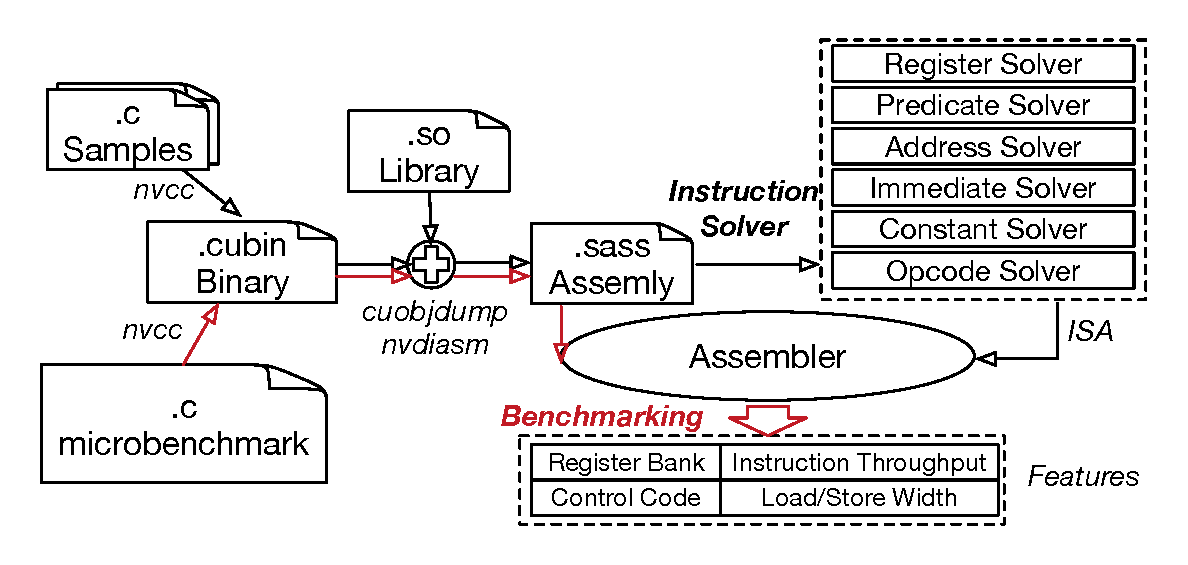
\includegraphics[scale=0.45]{methodology}
\caption{A schematic diagram of demystifying GPU microarchitecture features by leveraging CUDA binary tools. The back arrows represent the workflow of instruction solver while the red ones represents that of benchmarking to find out correlation between microarchitecture and performance.}
\label{fig:workflow}
\end{center}
\end{figure}

\subsection{Instruction Solver}
An instruction is composed of three main fields: {\tt opcode}, {\tt operands} and {\tt modifiers}.
%{\tt Operand} is composed of source operand and destination operand. Each kind of
Operands can be registers, constant memory, global memory, shared memory, immediate, or predicate register.
The encoding of operands can be inferred by their names. For instance, encoding of register operand {\tt R5} could be
inferred as $101$ by its binary, immediate $0x9$'s encoding could be $1001$. Besides, these fields are fixed length. For this kind of
fields, we could use Algorithm~\ref{algo:int_solver} to determine their positions and lengths and hence encoding.
NVIDIA document~\cite{cubin2015util} lists $94$ instructions of Kepler.
Each instruction can specify modifiers~\cite{ptx2015isa}, modifier defines different behaviours for same instruction. For example,
{\tt LD} instruction has type-size modifiers, such as .u8, .s8, .u16, .32, .64 and .128. {\tt LD} also has cache operation
modifier, such as .ca(cache at all level) and .cg(cache at global level).
Encodings of opcode and modifier are mnemonic symbols, we can not infer encoding by their names. Modifiers are instruction
specific, the same kind of modifier can be different encodings for different instructions. For instance, mask of type-size
modifier for {\tt LD} and {\tt LDG} are at different postions. So we deal with modifier for each instruction seperately.

\subsubsection{Operands:Fixed Length Field}
\begin{algorithm}
      \caption{Solver}
      \label{algo:int_solver}
  \begin{algorithmic}[1]
	  \State \textbf{input:} instmap
      \State output: pos, length
      \State currpos=\{\}
      \State prepos=\{0,1,2,...63\}
      \While {lenght(currpos) != 1}
      \State inst=instmap[random()]
      \If {inst.src1type == immediate}
      \State instencode=inst->encode64bit
      \State immbin = completecode(imm)
      \State pos = 0
      \While {pos + length(immbin) < 64}
      \If {strcmp(immbin,instencode+pos,length(immbin)}
      \State pushback(currpos, pos)
      \EndIf
      \EndWhile
      \State currpos = intersect (curpos, prepos)
      \State prepos = currpos
      \State currpos=\{\}
      \EndIf
      \EndWhile
      \State return curpos[0]
  \end{algorithmic}
\end{algorithm}
